\documentclass{beamer}
\mode<presentation>

\usepackage{amsmath, amssymb, multicol, mathtools}
\usepackage{listings} % For improved code formatting and line wrapping
\lstset{basicstyle=\scriptsize\ttfamily, breaklines=true} % Set font size and enable line wrapping

\usetheme{Boadilla}
\usecolortheme{lily}

\title{Directional and Normal Vectors of a Line}
\author{Bhukya Prajwal Naik \\ AI24BTECH11005}
\date{\today}

\setbeamertemplate{footline}{
  \leavevmode%
  \hbox{%
    \begin{beamercolorbox}[wd=\paperwidth,ht=2.25ex,dp=1ex,right]{author in head/foot}%
      \insertframenumber{} / \inserttotalframenumber\hspace*{2ex} 
    \end{beamercolorbox}}%
  \vskip0pt%
}
\setbeamertemplate{navigation symbols}{}

\newcommand{\myvec}[1]{\begin{pmatrix}#1\end{pmatrix}}

\begin{document}

\begin{frame}
  \titlepage
\end{frame}

\section*{Outline}
\begin{frame}{Outline}
  \tableofcontents
\end{frame}

\section{Problem}
\begin{frame}
  \frametitle{Problem Statement}
  \textbf{Question}: Find the directional and normal vectors of the line given by:
  \begin{align}
    x + y = 4
  \end{align}
\end{frame}

\section{Solution}
\subsection{Setting Up the Equation}
\begin{frame}
  \frametitle{Setting Up the Equation}
  The equation of the line can be rearranged as follows:
  \begin{align}
    x + y &= 4 \\
    y &= 4 - x
  \end{align}
  We can express the line in vector form:
  \begin{align}
   \myvec{x \\ y} &= \myvec{0 \\ 4} + x \myvec{1 \\ -1}
  \end{align}
  Here, we identify:
  \begin{itemize}
    \item A point on the line: \( \myvec{0 \\ 4} \)
    \item The direction vector: \( \myvec{1 \\ -1} \)
  \end{itemize}
\end{frame}

\subsection{Directional and Normal Vectors}
\begin{frame}
  \frametitle{Directional and Normal Vectors}
  From the vector form, we find:
  \begin{align}
    \text{Direction vector, } m &= \myvec{1 \\ -1} \\
    \text{Normal vector, } n &= \myvec{1 \\ 1}
  \end{align}

  \begin{table}[h!]
    \centering
    \begin{tabular}{|c|c|}
      \hline
      \textbf{Element} & \textbf{Mathematical Representation} \\
      \hline
      Given Line & \( X = h + km \) \\
      \hline
      Direction vector & \( m = \myvec{1 \\ -1} \) \\
      \hline
      Normal vector & \( n = \myvec{1 \\ 1} \) \\
      \hline
    \end{tabular}
    \caption{Results}
    \label{tab:info}
  \end{table}
\end{frame}

\begin{frame}{Vector Plot}
  \frametitle{Visual Representation}
  \begin{figure}
    \centering
    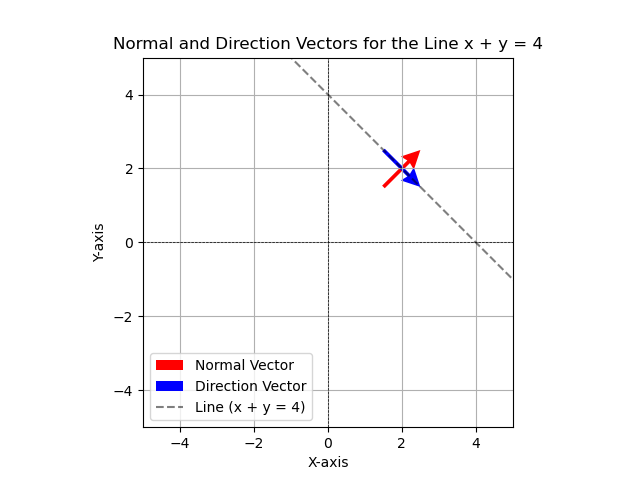
\includegraphics[width=0.5\linewidth]{Figures/Figure_1.png}
    \caption{Directional and Normal Vectors of the Line}
    \label{fig:vectors}
  \end{figure}

  The code at 
  \url{https://github.com/Prajwal-code77/EE1030/blob/main/presentations/codes/plot_vectors.py} 
  verifies equations (5) and (6).
\end{frame}

\section{Codes}
\subsection{C Code for Calculating Vectors}

\begin{frame}[fragile]
\frametitle{C Code}
\lstset{basicstyle=\tiny\ttfamily, breaklines=true}
\begin{lstlisting}
// vector_calculator.c
#include <stdio.h>

int main() {
    // Normal vector for the line x + y = 4
    int normal_vector[] = {1, 1}; // Coefficients of x and y
    // Direction vector, perpendicular to the normal vector
    int direction_vector[] = {1, -1}; // Any vector perpendicular to the normal

    // Output the vectors
    printf("Normal Vector: [%d, %d]\n", normal_vector[0], normal_vector[1]);
    printf("Direction Vector: [%d, %d]\n", direction_vector[0], direction_vector[1]);

    // Calculate and print line points
    printf("Line Points: ");
    for (int x = -8; x <= 8; x++) {
        int y = 4 - x; // y = 4 - x
        printf("[%d, %.2f]", x, (float)y); // Format to two decimal places
        if (x < 8) {
            printf(", "); // Add comma except for the last point
        }
    }
    printf("\n");

    return 0;
}
\end{lstlisting}
\end{frame}

\subsection{Plotting the Figure using Python}
\begin{frame}[fragile]
\frametitle{Plotting the Figure using Python}
\lstset{basicstyle=\tiny\ttfamily, breaklines=true}
\begin{lstlisting}
import matplotlib.pyplot as plt

# Normal and direction vectors
normal_vector = [1, 1]
direction_vector = [1, -1]
line_points = [(x, 4 - x) for x in range(-8, 9)]

x_line, y_line = zip(*line_points)
shifted_origin = [2, 2]

# Create the plot
plt.quiver(*shifted_origin, *normal_vector, color='r', angles='xy', scale_units='xy', scale=1, 
           width=0.01, headwidth=5, label='Normal Vector', pivot='middle')
plt.quiver(*shifted_origin, *direction_vector, color='b', angles='xy', scale_units='xy', scale=1, 
           width=0.01, headwidth=5, label='Direction Vector', pivot='middle')

plt.plot(x_line, y_line, 'k--', label='Line (x + y = 4)', alpha=0.5)  # Dashed line

plt.xlim(-5, 5)
plt.ylim(-5, 5)
plt.axhline(0, color='black', linewidth=0.5, ls='--')
plt.axvline(0, color='black', linewidth=0.5, ls='--')
plt.grid()
plt.title('Normal and Direction Vectors for the Line x + y = 4')
plt.xlabel('X-axis')
plt.ylabel('Y-axis')
plt.legend()
plt.gca().set_aspect('equal', adjustable='box')
plt.show()
\end{lstlisting}
\end{frame}

\end{document}
